\begin{enumerate}
	\item Exercício
	
	$R = \left\{(x, y) \in \mathbb{R}^2 \,|\, 0 \leq x \leq 2 \,,\, 0 \leq y \leq 6 \right\}$
	
	\begin{figure}[H]
		\centering
		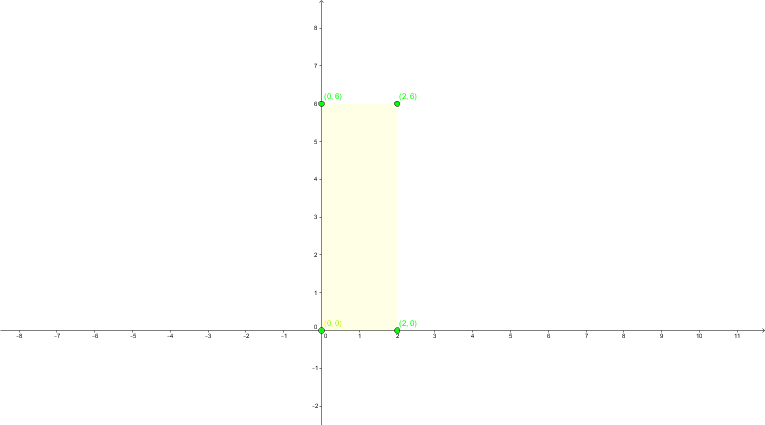
\includegraphics[width=\textwidth]{v01_a02_e01.png}
		\caption{Integrais duplas - Aula 2 - Exercício I}
		\label{v01_a02_e01}
	\end{figure}
	
	$\integral_0^2 dx \integral_0^6 dy = \integral_0^2 dx\, [y]_0^6 = \integral_0^2 dx\, [6 - 0] = 6\integral_0^2 dx = 6[x]_0^2 = 6[2 - 0] = 6 \cdot 2 = 12 $\newline
	
	\item Exercício
	
	$R = \left\{(x, y) \in \mathbb{R} \,|\, 0 \leq x \leq 1 \,,\, x \leq y \leq 2x \right\}$
						
	\begin{figure}[H]
		\centering
		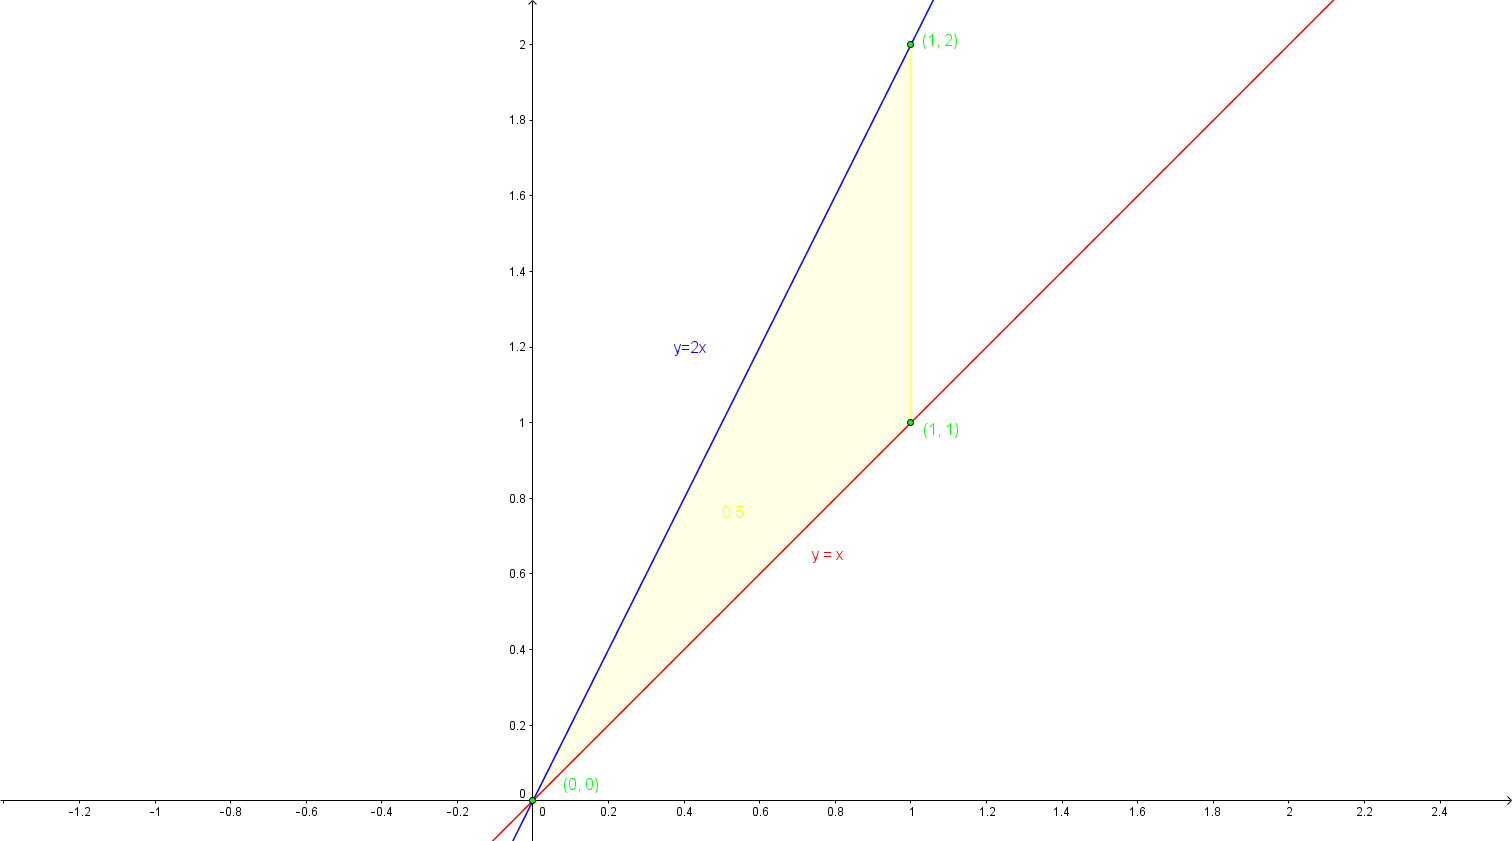
\includegraphics[width=\textwidth]{v01_a02_e02.png}
		\caption{Integrais duplas - Aula 2 - Exercício II}
		\label{v01_a02_e02}
	\end{figure}
	
	$\integral_0^1 dx \integral_{x}^{2x} dy = \integral_0^1 dx\, [y]_{x}^{2x} = \integral_0^1 dx\, [2x - x] = 2\integral_0^1 x\, dx - \integral_0^1 x\, dx = \left[\overstrike{2}\dfrac{x^2}{\overstrike{2}} - \dfrac{x^2}{2}\right]_0^1 = \left[\dfrac{2x^2 - x^2}{2}\right]_0^1 = \dfrac{1}{2}\left[x^2\right]_0^1 = \dfrac{1}{2}\left[1^2 \overstrike{- 0^2}\right] = \dfrac{1}{2} = 0,5 $\newline
	
	\item Exercício
	
	$R = \left\{(x, y) \in \mathbb{R}^2 \,|\, 0 \leq y \leq 1 \,,\, 0 \leq x \leq \sqrt{1 - y^2} \right\}$
	
	$y = 0,\, y=1$\newline
	$x = 0,\, x = \sqrt{1 - y^2} \Rightarrow x^2 = 1 - y^2 \Rightarrow x^2 - 1 = -y^2 \Rightarrow y^2 = -x^2 + 1 \Rightarrow y = \sqrt{1 -x^2}$
					
	\begin{figure}[H]
		\centering
		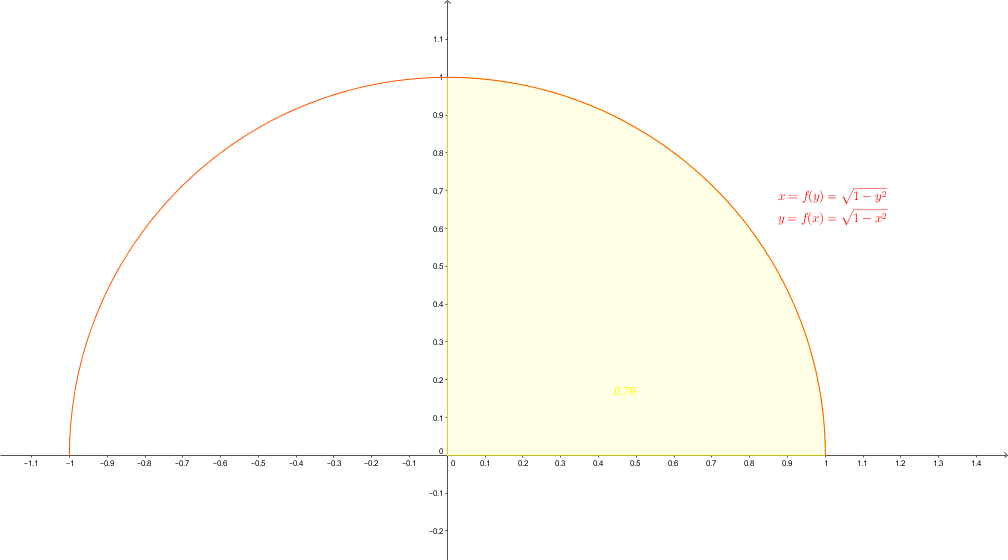
\includegraphics[width=\textwidth]{v01_a02_e03.png}
		\caption{Integrais duplas - Aula 2 - Exercício III}
		\label{v01_a02_e03}
	\end{figure}
	
	$\integral_0^1 dy \integral_0^{f(y)} dx = \integral_0^1 dy \integral_0^{\sqrt{1 - y^2}} dx = \integral_0^1 dy\, [x]_0^{\sqrt{1 - y^2}} = \integral_0^1 dy\, \left[\sqrt{1 - y^2} - 0\right] = \integral_0^1 \sqrt{1 - y^2}\, dy = \integral_0^1 \sqrt{1 - \sen^2(t)}\, \cos(t) dt = \integral_0^1 \sqrt{\cos^2(t)}\, \cos(t) dt = \integral_0^1 \cos(t)\cos(t) dt = \integral_0^1 \cos^2(t) dt = \integral_0^1 \dfrac{1 + \cos(2t)}{2} dt = \dfrac{1}{2}\integral_0^1 \left[1 + \cos(2t)\right] dt = \dfrac{1}{2}\integral_0^1 dt + \dfrac{1}{2}\integral_0^1 \cos(2t) dt = \dfrac{1}{2}\integral_0^1 dt + \dfrac{1}{2}\integral_0^1 \cos(u) \dfrac{du}{2} = \dfrac{1}{2}\integral_0^1 dt + \dfrac{1}{4}\integral_0^1 \cos(u)\, du = \left[\dfrac{1}{2}t + \dfrac{1}{4}\sen(u)\right]_0^1 = \left[\dfrac{t}{2} + \dfrac{\sen(2t)}{4}\right]_0^1 = \left[\dfrac{t}{2} + \dfrac{\overstrike{2}\sen(t)\cos(t)}{\overstrike{4}\,2}\right]_0^1 = \left[\dfrac{t + \sen(t)\cos(t)}{2}\right]_0^1 = \dfrac{1}{2}\left[\arcsen(y) + y\sqrt{1 - y^2}\right]_0^1 =\\ 
	\dfrac{1}{2}\left[\left(\arcsen(1) + \overstrike{1 \cdot\sqrt{1 - 1^2}}\right) - \left(\arcsen(0) \overstrike{+ 0 \cdot \sqrt{1 - 0^2}}\right)\right] = \dfrac{1}{2}\left[\dfrac{\pi}{2} - 0\right] = \dfrac{\pi}{4} = 0,785$ \newline\newline
	$y = \sen(t) \Rightarrow dy = \cos(t) dt$\newline
	$u = 2t \Rightarrow \dfrac{du}{2} = dt$\newline\newline
	$\sen(t) = \dfrac{co}{h} = \dfrac{y}{1} = y$\newline
	$h^2 = co^2 + ca^2 \Rightarrow 1 = y^2 + ca^2 \Rightarrow ca = \sqrt{1 - y^2}$\newline
	$\cos(t) = \dfrac{ca}{h} = \dfrac{\sqrt{1 - y^2}}{1} = \sqrt{1 - y^2}$\newline
	$y = \sen(t) \Rightarrow t = \arcsen(y)$
	
	\item Exercício
	
	$y = x^2 + 1 ,\, y = -x^2 - 1 ;\; x = 1 ,\, x = -1$\newline
	$R = \left\{(x, y) \in \mathbb{R} \,|\, -1 \leq x \leq 1 \,,\, -x^2 - 1 \leq y \leq x^2 + 1 \right\}$
	
	\begin{figure}[H]
		\centering
		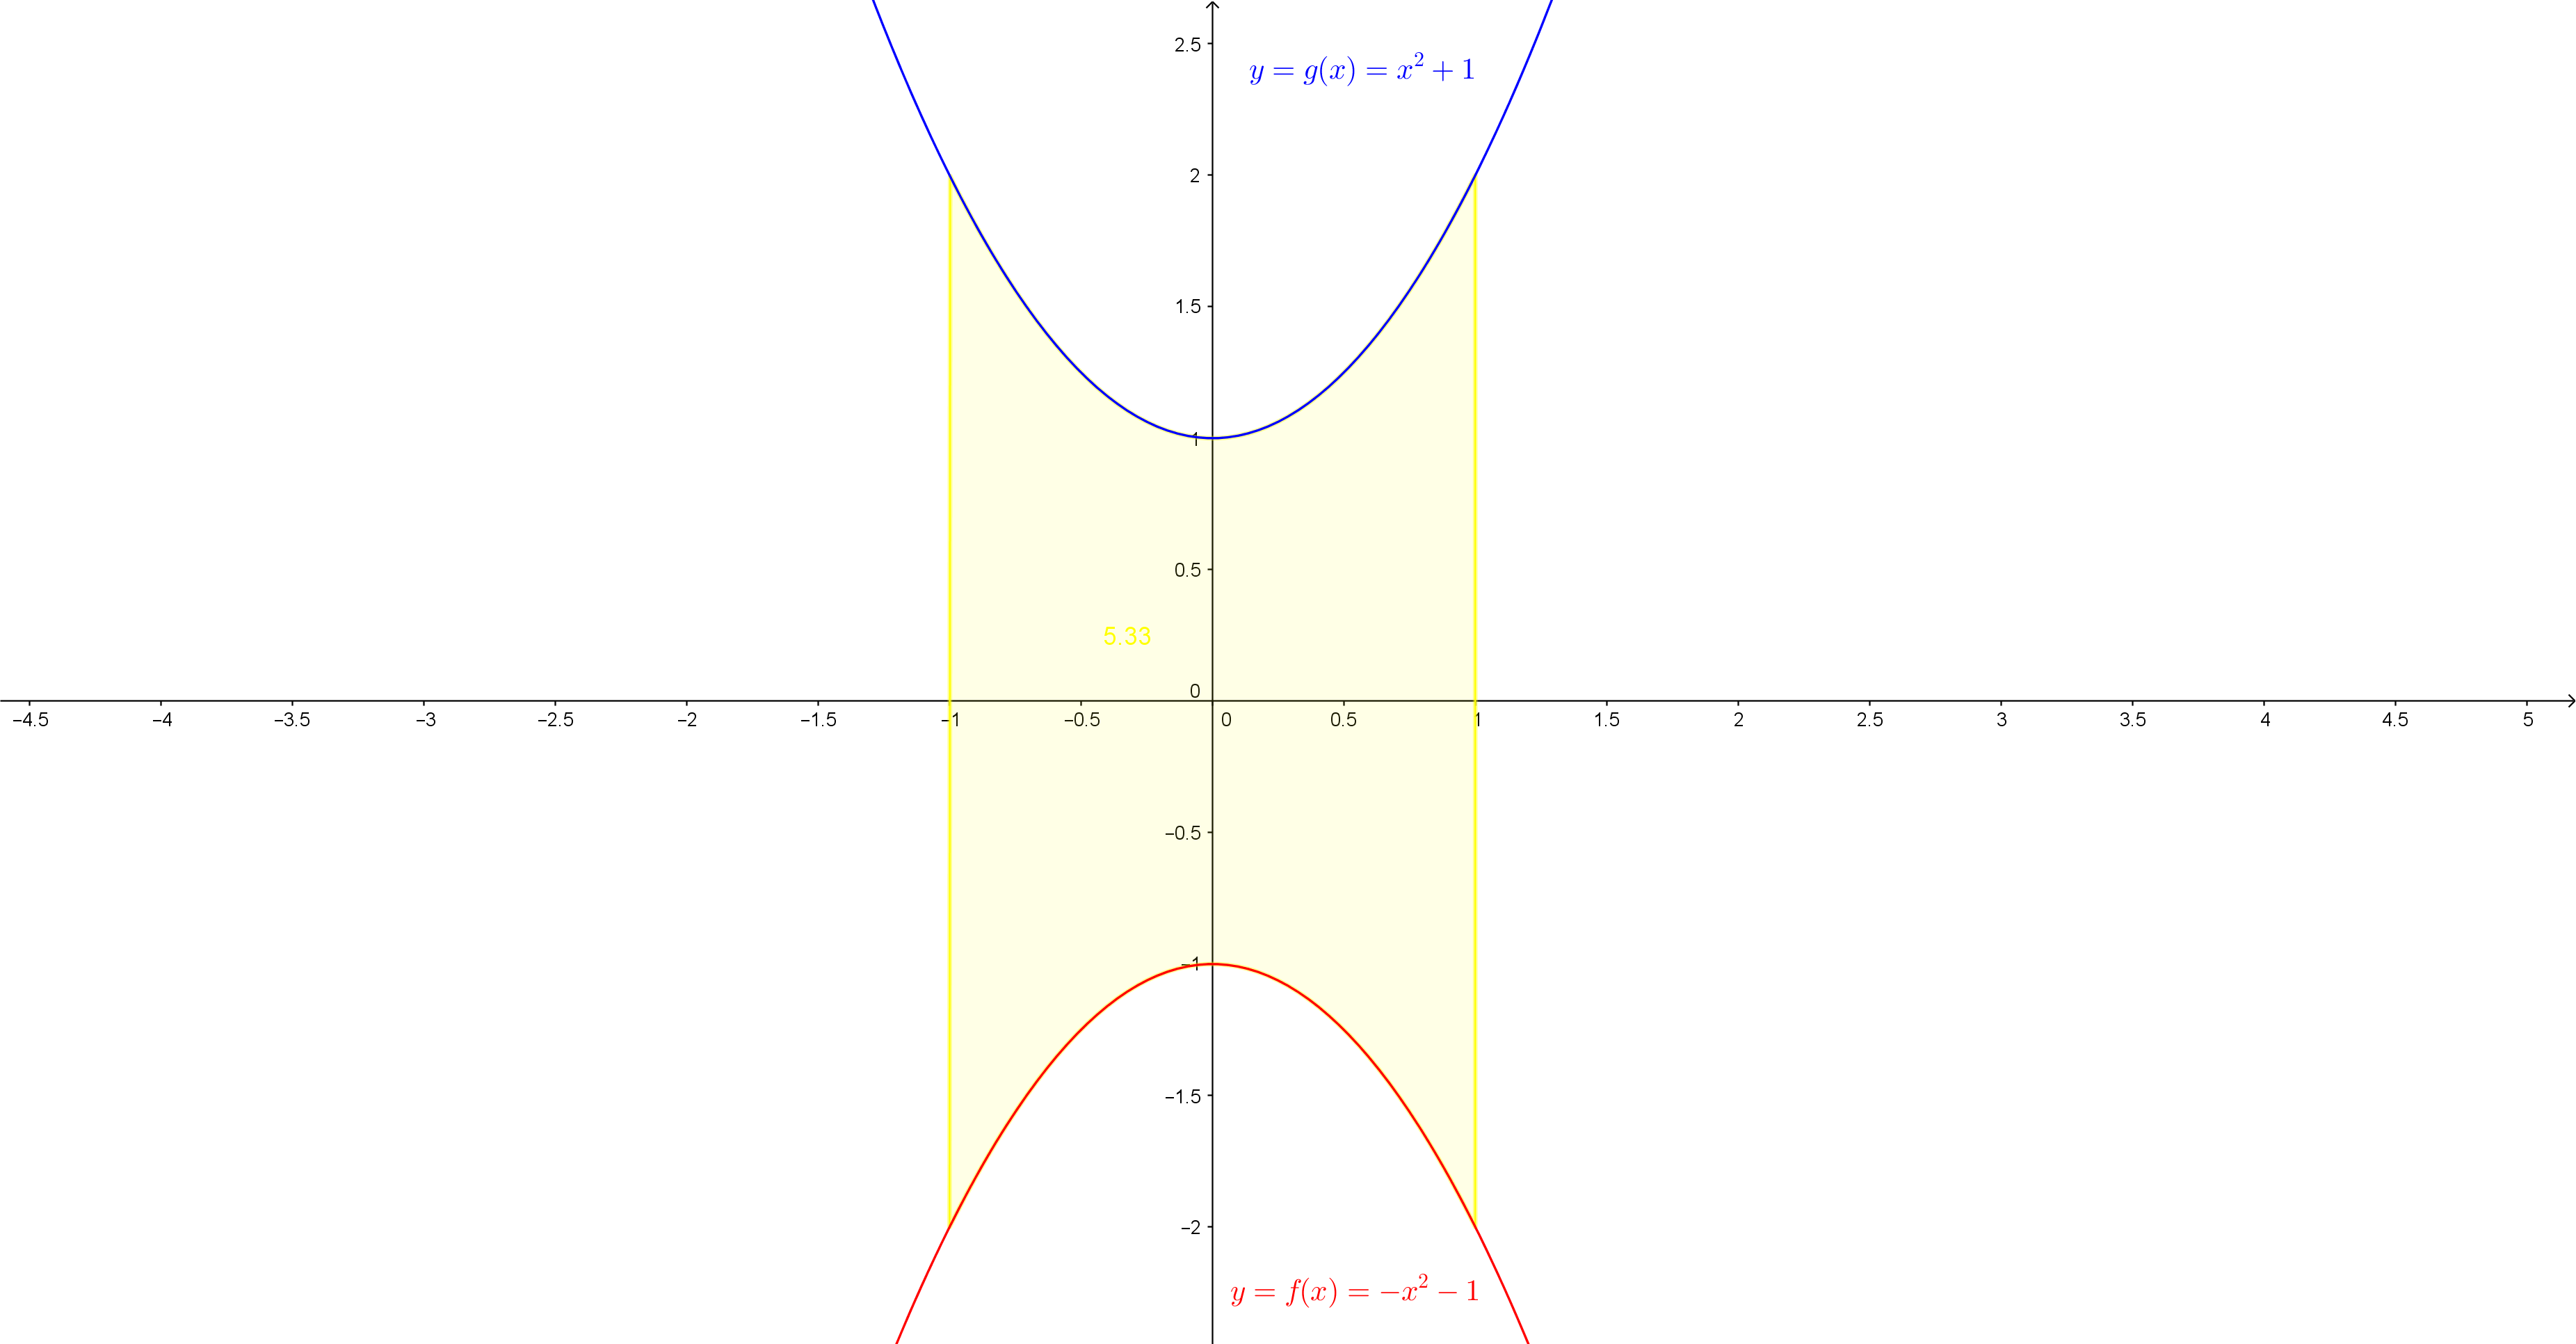
\includegraphics[width=\textwidth]{v01_a02_e04.png}
		\caption{Integrais duplas - Aula 2 - Exercício IV}
		\label{v01_a02_e04}
	\end{figure}
	
	$\integral_{-1}^1 dx \integral_{f(x)}^{g(x)} dy = \integral_{-1}^1 dx \integral_{-x^2 - 1}^{x^2 + 1} dy = \integral_{-1}^1 dx\, [y]_{-x^2 - 1}^{x^2 + 1} = \integral_{-1}^1 dx\, \left[x^2 + 1 - \left(-x^2 - 1\right)\right] = \integral_{-1}^1 dx\, \left[x^2 + 1 + x^2 + 1\right] = \integral_{-1}^1 dx\, \left[2x^2 + 2\right] = 2\integral_{-1}^1 x^2\, dx + 2\integral_{-1}^1 dx = \left[2\dfrac{x^3}{3} +  2x\right]_{-1}^1 = \left[2\left(\dfrac{x^3 + 3x}{3}\right)\right]_{-1}^1 = \dfrac{2}{3}\left[x\left(x^2 + 3\right)\right]_{-1}^1 = \\ 
	\dfrac{2}{3}\left[1 \cdot \left(1^2 + 3\right) - (-1)\left((-1)^2 + 3\right)\right] = \dfrac{2}{3}(4 + 4) = \dfrac{2}{3}8 = \dfrac{16}{3} = 5,\overline{3}$
	
	\item Exercício
	
	$R = \left\{(x, y) \in \mathbb{R} \,|\, 0 \leq y \leq 2 \,,\, -y \leq x \leq y \right\}$
	
	\begin{figure}[H]
		\centering
		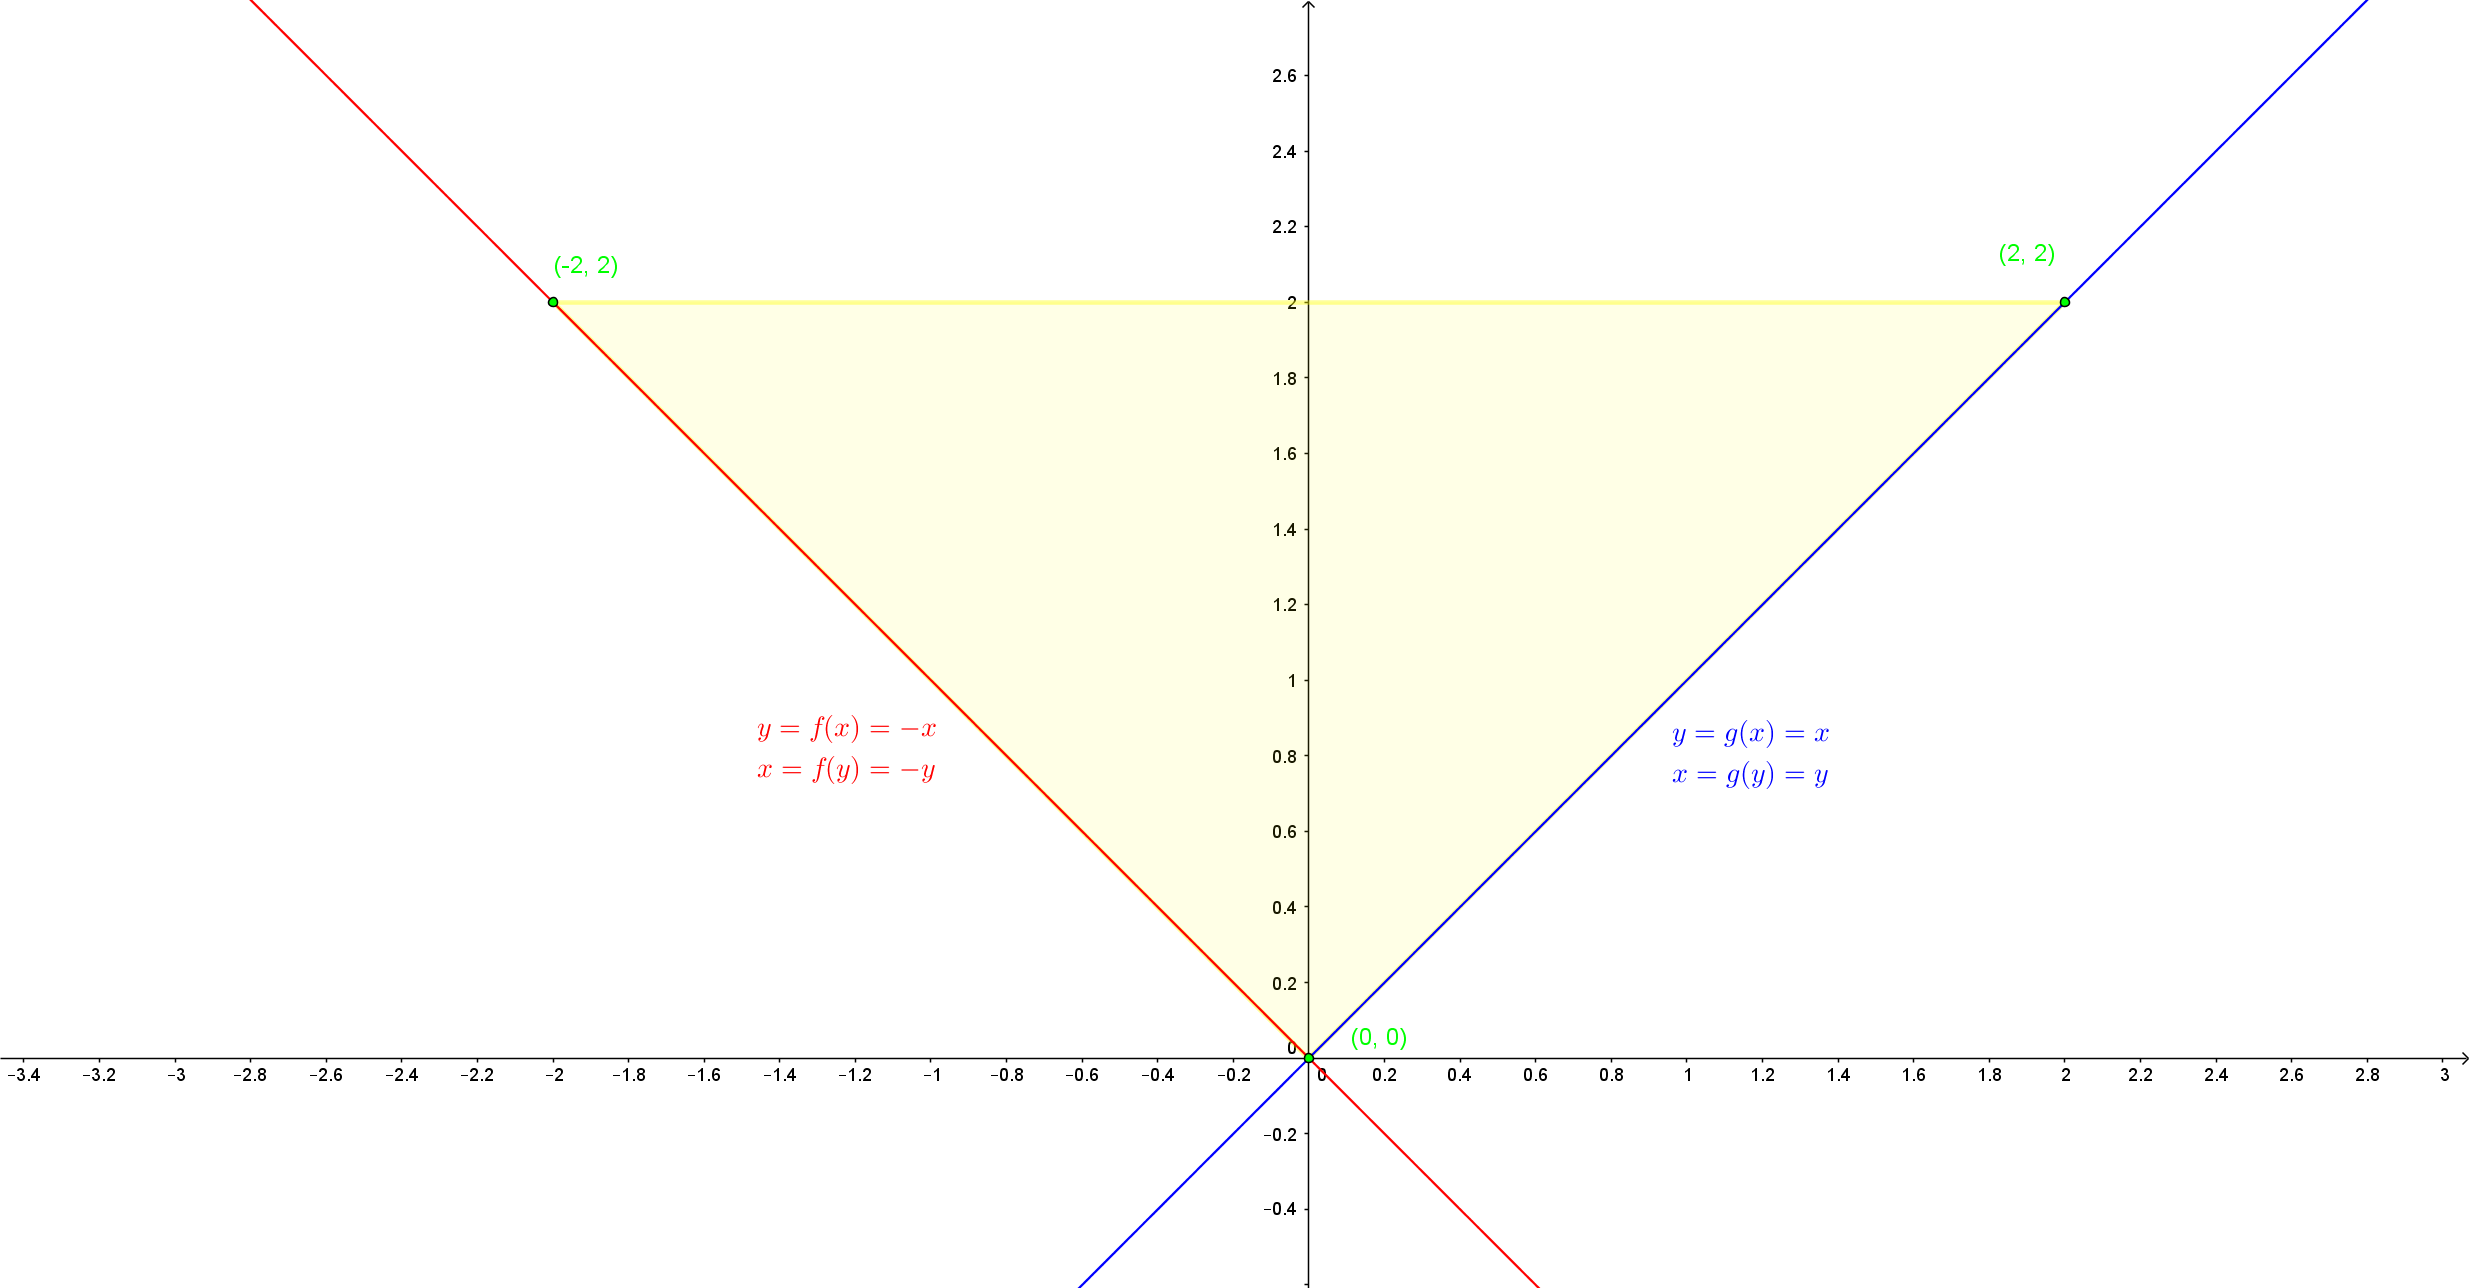
\includegraphics[width=\textwidth]{v01_a02_e05.png}
		\caption{Integrais duplas - Aula 2 - Exercício V}
		\label{v01_a02_e05}
	\end{figure}
	
	$\integral_0^2 dy \integral_{f(y)}^{g(y)} dx = \integral_0^2 dy \integral_{-y}^y dx = \integral_0^2 dy\, [x]_{-y}^y = \integral_0^2 dy\, [y - (-y)] = \integral_0^2 dy\, [2y] = 2\integral_0^2 y\, dy = \left[\overstrike{2}\frac{y^2}{\overstrike{2}}\right]_0^2 = 2^2 - 0^2 = 4$	
\end{enumerate}